\documentclass[journal,12pt,twocolumn]{IEEEtran}
%

\usepackage{setspace}
\usepackage{gensymb}
\singlespacing

\usepackage{amsmath}
\usepackage{amsthm}
\usepackage{txfonts}
\usepackage{cite}
\usepackage{enumitem}
\usepackage{mathtools}
\usepackage{listings}
    \usepackage{color}                                            %%
    \usepackage{array}                                            %%
    \usepackage{longtable}                                        %%
    \usepackage{calc}                                             %%
    \usepackage{multirow}                                         %%
    \usepackage{hhline}                                           %%
    \usepackage{ifthen}                                           %%
  %optionally (for landscape tables embedded in another document): %%
    \usepackage{lscape}     
\usepackage{multicol}
\usepackage{chngcntr}
\usepackage{float}
\renewcommand\thesection{\arabic{section}}
\renewcommand\thesubsection{\thesection.\arabic{subsection}}
\renewcommand\thesubsubsection{\thesubsection.\arabic{subsubsection}}

\renewcommand\thesectiondis{\arabic{section}}
\renewcommand\thesubsectiondis{\thesectiondis.\arabic{subsection}}
\renewcommand\thesubsubsectiondis{\thesubsectiondis.\arabic{subsubsection}}

% correct bad hyphenation here
\hyphenation{op-tical net-works semi-conduc-tor}
\def\inputGnumericTable{}                                 %%

\lstset{
%language=C,
frame=single, 
breaklines=true,
columns=fullflexible
}

\begin{document}
%


\newtheorem{theorem}{Theorem}[section]
\newtheorem{problem}{Problem}
\newtheorem{proposition}{Proposition}[section]
\newtheorem{lemma}{Lemma}[section]
\newtheorem{corollary}[theorem]{Corollary}
\newtheorem{example}{Example}[section]
\newtheorem{definition}[problem]{Definition}
\newcommand{\BEQA}{\begin{eqnarray}}
\newcommand{\EEQA}{\end{eqnarray}}
\newcommand{\define}{\stackrel{\triangle}{=}}
\bibliographystyle{IEEEtran}
\providecommand{\mbf}{\mathbf}
\providecommand{\pr}[1]{\ensuremath{\Pr\left(#1\right)}}
\providecommand{\qfunc}[1]{\ensuremath{Q\left(#1\right)}}
\providecommand{\sbrak}[1]{\ensuremath{{}\left[#1\right]}}
\providecommand{\lsbrak}[1]{\ensuremath{{}\left[#1\right.}}
\providecommand{\rsbrak}[1]{\ensuremath{{}\left.#1\right]}}
\providecommand{\brak}[1]{\ensuremath{\left(#1\right)}}
\providecommand{\lbrak}[1]{\ensuremath{\left(#1\right.}}
\providecommand{\rbrak}[1]{\ensuremath{\left.#1\right)}}
\providecommand{\cbrak}[1]{\ensuremath{\left\{#1\right\}}}
\providecommand{\lcbrak}[1]{\ensuremath{\left\{#1\right.}}
\providecommand{\rcbrak}[1]{\ensuremath{\left.#1\right\}}}
\theoremstyle{remark}
\newtheorem{rem}{Remark}
\newcommand{\sgn}{\mathop{\mathrm{sgn}}}
\providecommand{\abs}[1]{\left\vert#1\right\vert}
\providecommand{\res}[1]{\Res\displaylimits_{#1}} 
\providecommand{\norm}[1]{\left\lVert#1\right\rVert}
\providecommand{\mtx}[1]{\mathbf{#1}}
\providecommand{\mean}[1]{E\left[ #1 \right]}
\providecommand{\fourier}{\overset{\mathcal{F}}{ \rightleftharpoons}}
\providecommand{\system}{\overset{\mathcal{H}}{ \longleftrightarrow}}


\newcommand{\myvec}[1]{\ensuremath{\begin{pmatrix}#1\end{pmatrix}}}
\newcommand{\cmyvec}[1]{\ensuremath{\begin{pmatrix*}[c]#1\end{pmatrix*}}}
\newcommand{\mydet}[1]{\ensuremath{\begin{vmatrix}#1\end{vmatrix}}}
\newcommand{\proj}[2]{\textbf{proj}_{\vec{#1}}\vec{#2}}
\let\StandardTheFigure\thefigure
\let\vec\mathbf
\title{
ASSIGNMENT 6
}
\author{Gayathri S}
	

\maketitle
\renewcommand{\thefigure}{\theenumi}
\renewcommand{\thetable}{\theenumi}
  Download all python codes from 
\begin{lstlisting}
https://github.com/Gayathri1729/SRFP/tree/main/Assignment6
\end{lstlisting}
%
and latex-tikz codes from 
%
\begin{lstlisting}
https://github.com/Gayathri1729/SRFP/tree/main/Assignment6
\end{lstlisting}
%
\section{Quadratic Forms-2.74 j}
In each of the following, find the equation for
the ellipse that satisfies the given conditions:

Foci $\myvec{0 \\ \pm \sqrt{10}}$ , passing through $\myvec{2\\3}$.

\section{Solution}
The general equation of ellipse is
\begin{equation}
    \vec{x}^{\top}\vec{V}\vec{x} = 1
\end{equation}
where
\begin{equation}
    \vec{V} = \myvec{\lambda_1 & 0 \\ 0 & \lambda_2}
\end{equation} 
Given the ellipse is passing through $\myvec{2\\3}$ .

\begin{align}
   \Longrightarrow  \myvec{2&3}\vec{V} \myvec{2\\3}& = 1\\
     \myvec{2&3}\myvec{\lambda_1&0\\0&\lambda_2} \myvec{2\\3}& = 1
\end{align}
\begin{equation}
     \Longrightarrow 4\lambda_1 +9\lambda_2=1 \label{eq:5}
\end{equation}
Note that $\lambda_1$ $>$ $\lambda_2$.

Given the focus is $\myvec{0 \\ c}$= $\myvec{0 \\ \pm \sqrt{10}}$.Thus, the major axis of the ellipse is y-axis.
We know that for the ellipse whose major axis in y-axis,
\begin{equation}
    c^2=\frac{1}{\lambda_2}-\frac{1}{\lambda_1}
\end{equation}
\begin{equation}
     10=\frac{1}{\lambda_2}-\frac{1}{\lambda_1} \label{eq:7}
\end{equation}
From (\ref{eq:5})
\begin{equation}
    \lambda_2 = \frac{1-4\lambda_1 }{9}
\end{equation}
From (\ref{eq:7})
\begin{equation}
    \lambda_2 = \frac{\lambda_1 }{10\lambda_1 + 1}
\end{equation}
\begin{align}
  \Longrightarrow  \frac{1-4\lambda_1 }{9}&=\frac{\lambda_1 }{10\lambda_1 + 1}\\
  40\lambda_1^{2}+3\lambda_1-1&=0\\
  \lambda_1&=\frac{1}{8}
\end{align}
From (\ref{eq:5}),
\begin{equation}
    \lambda_2=\frac{1}{18}
\end{equation}
Thus the equation of the given ellipse is
\begin{equation}
    \vec{x}^{\top}\myvec{\frac{1}{8}&0\\0&\frac{1}{18}}\vec{x} = 1
\end{equation}
Fig \ref{fig:1} represents the given ellipse.
\numberwithin{figure}{section}
\begin{figure}[!ht]
\centering
    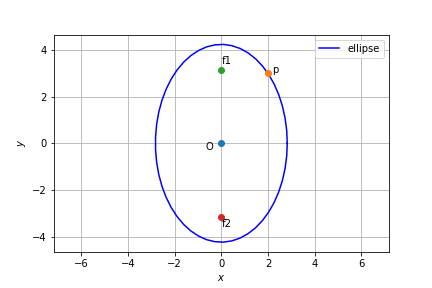
\includegraphics[width= \columnwidth]{assignment6.png}
    \caption{Ellipse} \label{fig:1}
\end{figure}
\end{document}